% ============================================================

%  Beamer Presentation Template

%  Deep Learning — Plaksha University

% ============================================================

\documentclass[12pt]{beamer}

% ---- Slide Dimensions & Geometry ---------------------------

% Set slide canvas to a widescreen 16:9 aspect ratio.

% 300mm x 168.75mm uses a 16:9 canvas, fitting dense content effortlessly.

\geometry{paperwidth=300mm, paperheight=168.75mm}

\setbeamersize{text margin left=10mm, text margin right=10mm}

% ---- Theme & Colour ----------------------------------------

\usetheme{Madrid}

\usecolortheme{default}

% Uncomment one of the alternatives below:

% \usetheme{metropolis}

% \usetheme{AnnArbor}

% \usecolortheme{dolphin}

\setbeamertemplate{navigation symbols}{}   % hide nav icons

% ---- Packages ----------------------------------------------

\usepackage{amsmath, amssymb, amsthm}

\usepackage{graphicx}

\usepackage{booktabs}          % \toprule / \midrule / \bottomrule

\usepackage{hyperref}

\usepackage{xcolor}

\usepackage{listings}          % code blocks

\usepackage{algorithm2e}       % pseudocode

\usepackage{tikz}              % diagrams (optional)
\usetikzlibrary{arrows.meta}
\usepackage{colortbl}          % enables \rowcolor

\usepackage{caption}

\usepackage{subcaption}

% Figures are loaded normally when the local figures/ folder exists.
% During standalone compilation, absent figures are shown as placeholders.
\newcommand{\maybegraphic}[2][]{%
  \IfFileExists{#2}{\includegraphics[#1]{#2}}{%
    \fbox{\parbox[c][2.5cm][c]{0.68\linewidth}{\centering\scriptsize
      Figure unavailable here:\\[1mm]\texttt{\detokenize{#2}}}}%
  }%
}

\definecolor{navy}{HTML}{162E52}

\definecolor{steel}{HTML}{3A6893}

\definecolor{lightblue}{HTML}{E7F0FA}

\definecolor{lavender}{HTML}{F0EBFA}

\definecolor{mint}{HTML}{E7F6EF}

\definecolor{ink}{HTML}{263343}

% ---- Listings (code) style ---------------------------------

\lstset{
basicstyle=\ttfamily\small,
keywordstyle=\color{blue},
commentstyle=\color{gray},
stringstyle=\color{orange},
numbers=left,
numberstyle=\tiny\color{gray},
breaklines=true,
frame=single
}

% ---- Metadata ----------------------------------------------

\title[PINNs in Unsteady Flows]{Using PINNs to overcome temporal and spatial sparsity in unsteady flows}

\subtitle{Deep Learning}

\author[Group 42]{Avani Mahawar, Gautam Ganesh, Esraaj Sarkar Gupta, Shikhraj Singh}

\institute[Plaksha]{Plaksha University}

\date{\today}

% ============================================================

\begin{document}

% ============================================================

% ---- Title slide -------------------------------------------

\begin{frame}

  \titlepage

\end{frame}

% ============================================================

\section{Introduction and Motivation}

% ============================================================

\begin{frame}{Introduction and Motivation}

  \begin{itemize}

    \item Obtaining high-resolution fluid-flow data is expensive: cameras have \textbf{finite acquisition rates} and \textbf{spatial resolution is limited} by optical access and particle density.

    \item \textbf{Computational Limitations} also exist: When generating flow fields using CFD, high resolution simulations can contain millions of spatial cells over thousands of temporal snapshots.

    \item It is essential to understand the entire flow to model relevant quantities --- forces, energy losses, flow stability, etc. --- which depend on the entire flow, as opposed to just the few points where measurements are available.

  \end{itemize}

  \begin{alertblock}{Interpolation}

      Conventional linear interpolation fails at this task, proving only reasonable when the flow varies smoothly and ``sufficiently'' slowly between observations.  

  \end{alertblock}

  \begin{figure}

    \centering

    \maybegraphic[width=0.35\textwidth]{figures/interpolation.png}

    \caption{Data EDA: Linear Interpolation Errors (more on this in the following slides)}

  \end{figure}

\end{frame}

% ---- Two-column slide example ------------------------------

\begin{frame}{Introduction and Motivation: Using PINNs}

  \begin{columns}[T,onlytextwidth]

    \begin{column}{0.48\textwidth}

      Why does domain literature suggest PINNs?

      \begin{itemize}

        \item When the temporal sampling rate is insufficient, different oscillatory signals can produce identical observations.

        \item While no reconstruction method can universally recover fundamentally unidentifiable information, PINNs can introduce additional physical constraints.

        \item If a PINN returns a continuous function $(u, v, p) = \mathcal{N}(x,y,t)$, it can be evaluated at any arbitrary spatio-temporal coordinates. This reduces hardware space required to store results.

      \end{itemize}

    \end{column}

    \begin{column}{0.48\textwidth}

      \begin{alertblock}{The Navier--Stokes Equations}

        The Navier--Stokes equations provide additional constraints. The flow must approximately satisfy:

\[
\begin{aligned}
\frac{\partial \mathbf{u}}{\partial t}+(\mathbf{u}\cdot\nabla)\mathbf{u}
 &= -\nabla p+\frac{1}{Re}\nabla^2\mathbf{u},\\
\nabla\cdot\mathbf{u}&=0.
\end{aligned}
\]

        These equations restrict the possible velocity fields that can exist between observations.

      \end{alertblock}

    \end{column}

  \end{columns}

  {\tiny\color{steel}Sources: Raissi et al., J. Comput. Phys. 378 (2019); Sundar et al., arXiv:2503.15679 (2025).}

\end{frame}

% ============================================================

\section{Data}

% ============================================================

\begin{frame}{Dataset \& Exploratory Data Analysis}

  \begin{columns}[T]

    \begin{column}{0.53\textwidth}

      \begin{block}{Open-Source Data: Boudina \textit{et al.}}

        2D finite element simulation of a fixed circular cylinder at

$Re = 100$ (laminar, periodic vortex shedding). Generated using an

        in-house solver for CFD and Fluid-Structure Interaction (FSI).

      \end{block}

      \vspace{0.5em}

      \begin{block}{Exploratory Data Analysis (EDA)}

        \textbf{Scale \& Geometry:}

        \begin{itemize}

          \item $82,872$ spatial nodes over $201$ temporal snapshots ($\approx 16.66\times 10^6$ records).

          \item Three flow zones: cylinder wall ($628$ nodes), near-body ($24,250$ nodes), wake ($18,977$ nodes).

          \item Training crop ($x \in [-1.5, 8], y \in [-2, 2]$): $43,855$ nodes ($\approx 52.9\%$ of nodes in $<0.2\%$ area).

        \end{itemize}

        \vspace{0.3em}

        \textbf{Flow Dynamics:}

        \begin{itemize}

          \item Export spans $3.30$ shedding cycles ($t = 400 \to 420, \Delta t = 0.1$).

          \item Fully periodic K\'arm\'an street with period $T = 6.066\, D/U_0$ ($St = 0.165$).

          \item Phase-repeat consistency error $< 0.21\%$.

        \end{itemize}

        \vspace{0.2em}

        {\footnotesize ($D$: cylinder diameter; $U_0$: freestream velocity; $Re = U_0 D / \nu$)}

      \end{block}

    \end{column}

    \begin{column}{0.45\textwidth}

      \begin{figure}

        \centering

        \maybegraphic[width=\linewidth]{figures/data_example.png}

        \caption{Raw CFD export structure: Illustrative Example}

      \end{figure}

      \vspace{-0.5em}

      \begin{figure}

        \centering

        \maybegraphic[width=\linewidth]{figures/mesh.png}

        \caption{Full FEM mesh vs. near-body and wake crop}

      \end{figure}

    \end{column}

  \end{columns}

\end{frame}

\begin{frame}{Dataset \& Exploratory Data Analysis}

  \begin{figure}

        \centering

        \maybegraphic[width=0.80\textwidth]{figures/fields.png}

        \caption{Example field export}

  \end{figure}

\end{frame}

% ============================================================

\section{Methodology}

% ============================================================

\begin{frame}{Proposed Method}

\small

\textbf{Question:} How accurately can sparse cylinder-flow velocity measurements recover unobserved $(u,v)$ and pressure $p$?

\vspace{0.35cm}

\begin{columns}[T,onlytextwidth]

  \begin{column}{0.48\textwidth}

    \begin{block}{Completed pilot: spatial reconstruction}

      \begin{itemize}\setlength{\itemsep}{0.21cm}

        \item \textbf{Spatial interpolation:} Delaunay linear baseline.

        \item \textbf{Plain PINN:} MLP with data and physics losses.

        \item \textbf{Attention PINN:} attention across neighboring time-coordinate embeddings.

        \item \textbf{Segmented PINN:} four time windows, sequential weight transfer.

      \end{itemize}

    \end{block}

  \end{column}

  \begin{column}{0.48\textwidth}

    \begin{block}{Planned controlled experiments}

      \begin{itemize}\setlength{\itemsep}{0.21cm}

        \item Compare \textbf{temporal linear interpolation}, a \textbf{data-only ANN}, and PINNs.

        \item Vary \textbf{spatial sensor density} and \textbf{temporal observation gaps} independently.

        \item Use matched training budgets and test on unseen positions \emph{and} withheld times.

        \item Assess velocity, gauge-aligned pressure, and physics consistency.

      \end{itemize}

    \end{block}

  \end{column}

\end{columns}

\vspace{0.2cm}

{\footnotesize\color{steel}Current pilot: $Re=100$; 64 sensors from 43,855 nodes; 201 snapshots at $t\in[400,420]$. Data-only ANN and temporal-gap tests remain proposed.}

\end{frame}

% ---- Architecture diagram placeholder ----------------------

\begin{frame}{Architecture: Attention PINN (Implemented Variant)}

\centering

\vspace{0.12cm}

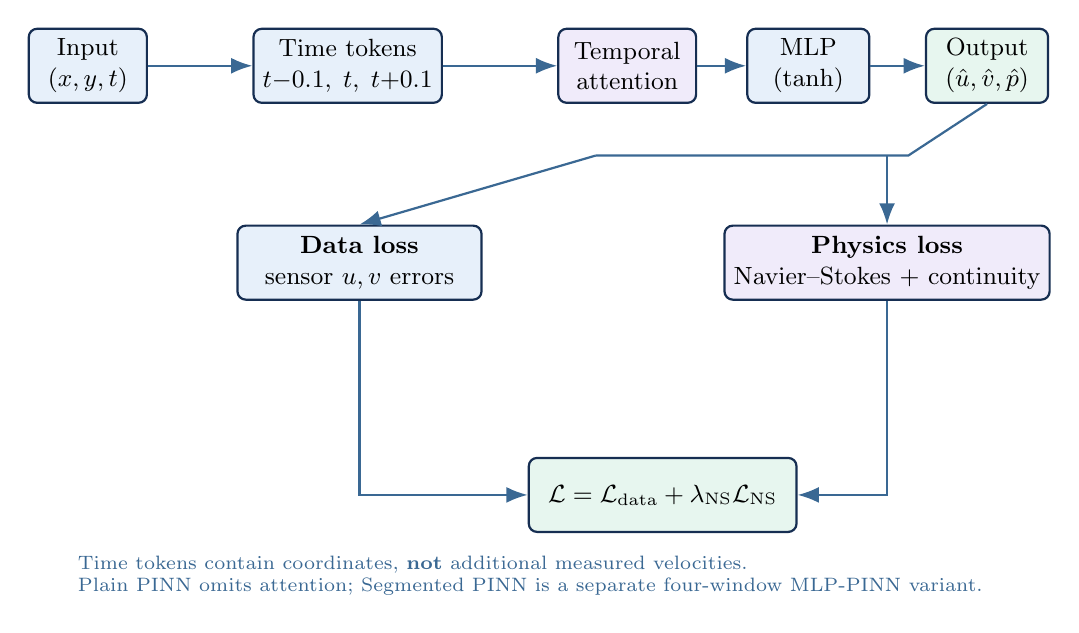
\begin{tikzpicture}[x=1cm,y=1cm,
    every node/.style={font=\small,align=center},
    box/.style={draw=navy,rounded corners=3pt,thick,minimum height=0.94cm,align=center},
    flow/.style={-{Latex[length=2.7mm]},thick,draw=steel}]
  \node[box,fill=lightblue,minimum width=1.5cm] (in) at (0,0) {Input\\$(x,y,t)$};
  \node[box,fill=lightblue,minimum width=2.1cm] (emb) at (3.3,0) {Time tokens\\$t{-}0.1,\;t,\;t{+}0.1$};
  \node[box,fill=lavender,minimum width=1.75cm] (att) at (6.85,0) {Temporal\\attention};
  \node[box,fill=lightblue,minimum width=1.55cm] (mlp) at (9.15,0) {MLP\\(tanh)};
  \node[box,fill=mint,minimum width=1.55cm] (out) at (11.42,0) {Output\\$(\hat u,\hat v,\hat p)$};
  \draw[flow] (in)--(emb);\draw[flow] (emb)--(att);\draw[flow] (att)--(mlp);\draw[flow] (mlp)--(out);
  \node[box,fill=lightblue,minimum width=3.1cm] (data) at (3.45,-2.5) {\textbf{Data loss}\\sensor $u,v$ errors};
  \node[box,fill=lavender,minimum width=3.55cm] (phys) at (10.15,-2.5) {\textbf{Physics loss}\\Navier--Stokes + continuity};
  \node[box,fill=mint,minimum width=3.4cm] (loss) at (7.3,-5.45) {$\mathcal L=\mathcal L_{\mathrm{data}}+\lambda_{\mathrm{NS}}\mathcal L_{\mathrm{NS}}$};
  \draw[draw=steel,thick] (out.south) -- (10.42,-1.14) -- (6.45,-1.14);
  \draw[flow] (6.45,-1.14) -- (data.north);
  \draw[flow] (10.15,-1.14) -- (phys.north);
  \draw[flow] (data.south) |- (loss.west);
  \draw[flow] (phys.south) |- (loss.east);
  \node[font=\scriptsize,align=left,text=steel,anchor=west] at (-0.25,-6.48) {Time tokens contain coordinates, \textbf{not} additional measured velocities.\\Plain PINN omits attention; Segmented PINN is a separate four-window MLP-PINN variant.};
\end{tikzpicture}

\vspace{0.10cm}

\begin{equation*}
\mathcal L_{\mathrm{NS}}=\left\langle \big\|\mathbf u_t+(\mathbf u\cdot\nabla)\mathbf u+\nabla p-\tfrac{1}{Re}\nabla^2\mathbf u\big\|^2+(u_x+v_y)^2\right\rangle.
\end{equation*}

\vspace{-0.15cm}

{\scriptsize\color{steel}No explicit boundary-condition loss or pressure labels are used during training in the current script.}

\end{frame}

% ============================================================

\section{Experiments}

% ============================================================


\begin{frame}{Experiments: Completed Pilot Results}

\small

\textbf{Cylinder wake, $Re=100$:} 64 sensor nodes; 43,791 held-out spatial nodes; 201 times, $t\in[400,420]$.\\

\textbf{Metric:} pooled relative $L^2$ error (\%), over all 201 snapshots.

\vspace{0.30cm}

\centering

\renewcommand{\arraystretch}{1.32}

\begin{table}
\centering
\small
\renewcommand{\arraystretch}{1.3}

\begin{tabular}{lrrrrr}
\toprule
\textbf{Method}
& \textbf{Parameters}
& \textbf{Steps}
& \textbf{$u$ (\%)}
& \textbf{$v$ (\%)}
& \textbf{$p$ (\%)} \\
\midrule

Spatial Delaunay interpolation
& ---
& ---
& 29.35
& 50.25
& --- \\

Plain PINN
& 8,771
& 10,000
& 25.47
& 85.72
& 49.96 \\

Attention PINN
& 21,251
& 10,000
& 26.57
& 86.94
& 51.17 \\

\rowcolor{mint}
\textbf{Segmented PINN}
& \textbf{4 $\times$ 8,771}
& \textbf{40,000}
& \textbf{20.64}
& \textbf{42.32}
& \textbf{48.33} \\

\bottomrule
\end{tabular}

\vspace{0.15cm}
{\scriptsize
Relative $L^2$ errors pooled over 201 snapshots.
Segmented PINN uses four subnetworks with 8,771 parameters each.
}
\end{table}

\vspace{0.06cm}

\begin{block}{Interpretation}

\begin{itemize}\setlength{\itemsep}{0.06cm}

  \item Segmentation has the lowest pooled errors, but received \textbf{$4\times$} the optimizer steps.

  \item Attention does \textbf{not} improve upon the plain PINN in this pilot.

  \item Spatial interpolation beats both global PINNs on $v$; segmented predictions jump at time-window boundaries.

\end{itemize}

\end{block}

\vspace{-0.07cm}

{\scriptsize\color{steel}Spatial holdout only; no withheld times. $p$ gauge-aligned per snapshot; interpolation predicts $(u,v)$ only.}

\end{frame}

% ============================================================

\section{References}

% ============================================================

\begin{frame}[allowframebreaks]{References}

  \IfFileExists{references.bib}{%
  \bibliographystyle{alpha}
  \bibliography{references}
}{%
  \begin{thebibliography}{9}
  \bibitem{raissi2019physics} M. Raissi, P. Perdikaris, G. E. Karniadakis,
  \emph{Journal of Computational Physics} 378 (2019), 686--707.
  \bibitem{sundar2025sequential} R. Sundar, D. Lucor, S. Sarkar,
  \emph{Sequential learning based PINNs}, arXiv:2503.15679 (2025).
  \end{thebibliography}
}

\end{frame}

% ============================================================

\end{document}
